%%%%%%%%%%%%%%%%%%%%%%%%%%%%%%%%%%%%%%%%%%%%%%%%%%%%%%%%%%%%%%%%%%%%%%%
% Universidade Federal de Santa Catarina             
% Departamento de Automação e Sistemas                    
%                                                           
% (c)2017	Andrei Donati
%           Ígor Assis Rocha Yamamoto
%           Luis Felipe Pelison
%           
%%%%%%%%%%%%%%%%%%%%%%%%%%%%%%%%%%%%%%%%%%%%%%%%%%%%%%%%%%%%%%%%%%%%%%%
\documentclass [12pt, a4paper] {article}
\usepackage{float}
\usepackage[utf8]{inputenc}
\usepackage[brazil]{varioref}
\usepackage{graphicx,epsfig,psfrag}
\usepackage{gensymb}
\usepackage{amssymb}
\usepackage{mathtools}
\usepackage{amsmath}
\usepackage[english,brazil]{babel}
\usepackage{indentfirst}
\usepackage{float}
\usepackage{color}
\usepackage{hyperref}
\usepackage{listings}
\graphicspath{{./fig/}}
%%%%%%%%%%%%%%%%%%%%%%%%%%%%%%%%%%%%%%%%%%%%%%%%%%%%%%%%%%%%%%%%%%%%%%%%
\begin{document}
%\patchcmd{\thebibliography}{\section*}{\section}{}{}
\begin{titlepage}
%%%%%%%%%%%%%%%%%%%%%%%%%%%%%%%%%%%%%%%%%%%%%%%%%%%%%%%%%%%%%%%%%%%%%%%%
%   ____                  
%  / ___|__ _ _ __   __ _ 
% | |   / _` | '_ \ / _` |
% | |__| (_| | |_) | (_| |
%  \____\__,_| .__/ \__,_|
%            |_|          

	\centering
	{\LARGE Universidade Federal de Santa Catarina \par}
	\vspace{4cm}
	{\Huge\bfseries Desenvolvimento de um controlador de caminhão usando Lógica Fuzzy\par}
	\vspace{1cm}
	{\scshape\Large INE5430 - Inteligência Artificial\par}
	\vspace{4cm}
	\emph{Alunos}\par
	{\large Andrei Donati \par}
	{\large Ígor Assis Rocha Yamamoto\par}
    {\large Luis Felipe Pelison\par}
    
	\vspace{1.5cm}
	\emph{Professor}\par
	{\large Mauro Roisenberg\par}

	\vfill
% Bottom of the page
	{\large Novembro de 2017\par}
\end{titlepage}

%%%%%%%%%%%%%%%%%%%%%%%%%%%%%%%%%%%%%%%%%%%%%%%%%%%%%%%%%%%%%%%%%%%%%%%%
%  ____
% / ___| _   _ _ __ ___   __ _ _ __(_) ___  
% \___ \| | | | '_ ` _ \ / _` | '__| |/ _ \ 
%  ___) | |_| | | | | | | (_| | |  | | (_) |
% |____/ \__,_|_| |_| |_|\__,_|_|  |_|\___/ 

\tableofcontents
\newpage
%%%%%%%%%%%%%%%%%%%%%%%%%%%%%%%%%%%%%%%%%%%%%%%%%%%%%%%%%%%%%%%%%%%%%%%%


\section{Introdução}
O seguinte trabalho propõe o desenvolvimento de um sistema de comando de autoparking para um caminhão usando lógica fuzzy e um código já desenvolvido e disponibilizado. O sistema está dividido em duas partes, no qual o foco é modificar apenas uma para que o caminhão consiga estacionar em uma doca de carregamento.


\newpage
\section{Sistema Fuzzy }
A lógica fuzzy é um tipo de lógica a qual permite que algumas verdades sejam parciais, ou seja, ela consegue representar quão bem algo se adequa a esta descrição. Desta forma, o sistema proposto pode ser modelado e controlado usando esta técnica. \par

O seguinte capítulo irá descrever o processo de modelagem e controle seguindo as técnicas abordadas durante as aulas da disciplina.

\subsection{Conjuntos}
Para transformar o sistema do caminhão + ambiente em algo computável foram selecionadas 3 variáveis consideradas como fundamentais: Posição no eixo X; Posição no eixo Y; Orientação do caminhão.\par
Dessa forma, a primeira variável (eixo X) foi fuzzyficada em três estados e pode ser vista no gráfico abaixo:

\begin{figure}[H]
    \centering
    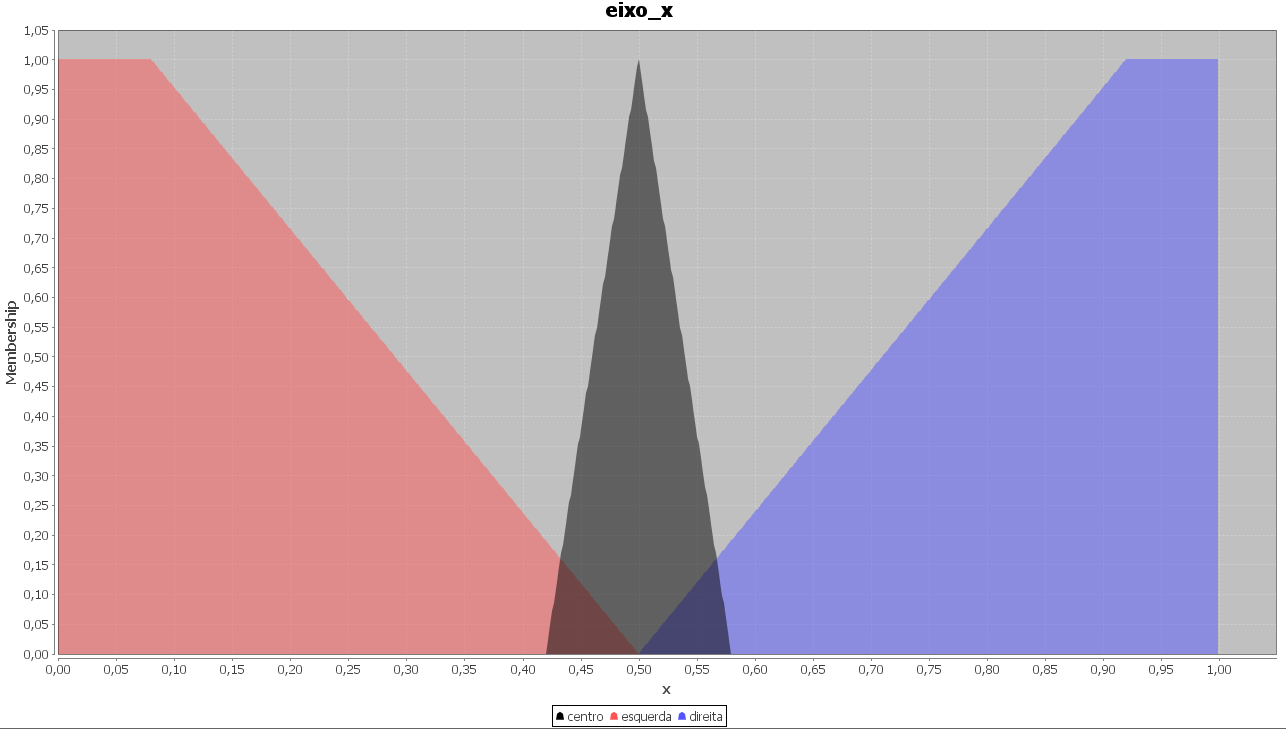
\includegraphics[width=\textwidth]{fig/eixo_x.png}
    \caption{Gráfico de fuzzyficação do eixo X}
    \label{fig:axioms}
\end{figure}
Estes conjuntos expressam o quão no centro, a esquerda ou a direita o caminhão está.

\begin{figure}[H]
    \centering
    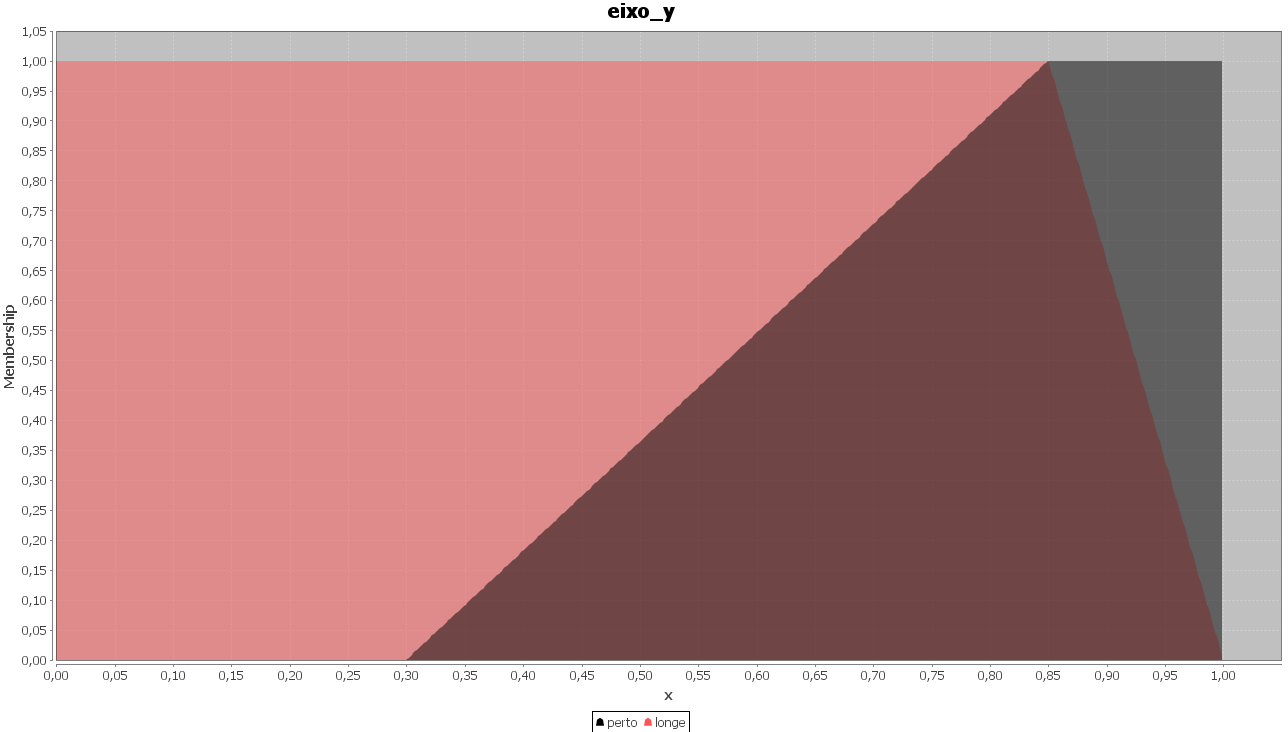
\includegraphics[width=\textwidth]{fig/eixo_y.png}
    \caption{Gráfico de fuzzyficação do eixo Y}
    \label{fig:axioms}
\end{figure}
Estes conjuntos expressam o quão longe, verticalmente, o caminhão está da doca. Como esta variável é menos crítica que a variável relacionada ao eixo x, apenas 2 estados fuzzy foram o suficiente para modela-la.

\begin{figure}[H]
    \centering
    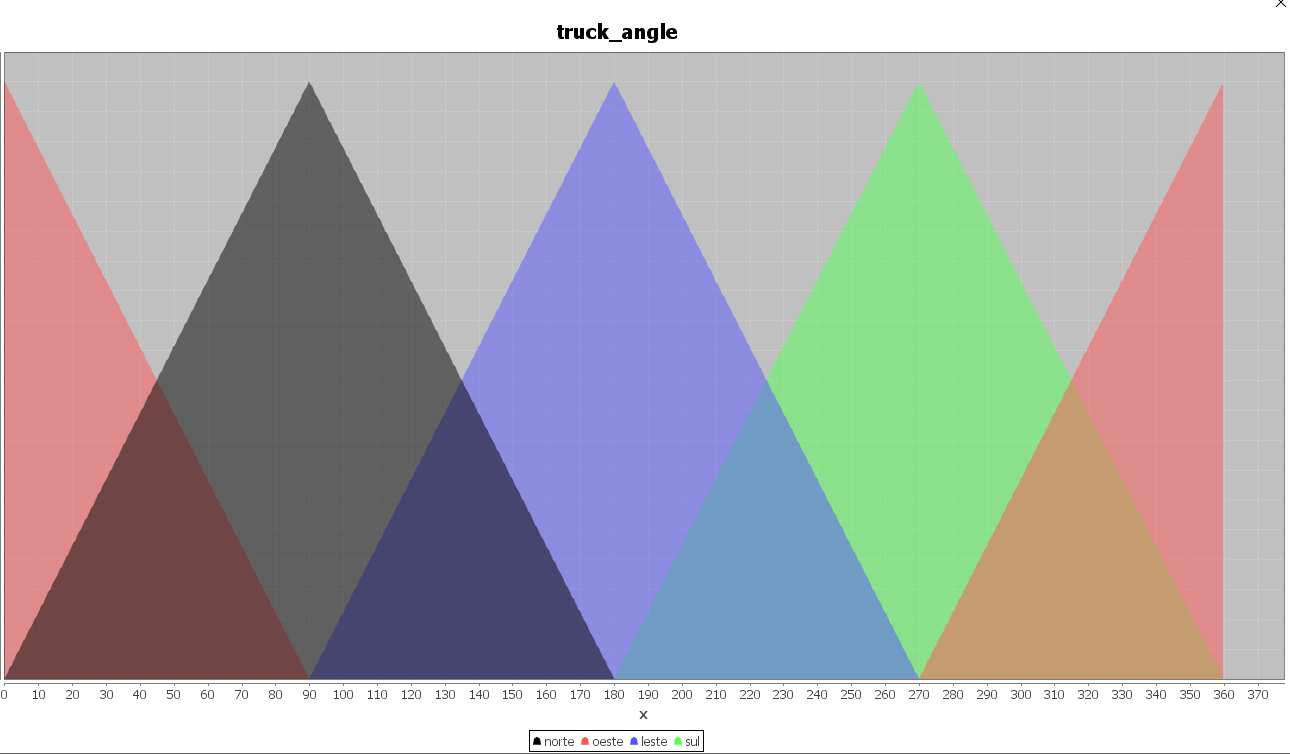
\includegraphics[width=\textwidth]{fig/truck_angle.png}
    \caption{Gráfico de fuzzyficação do ângulo do caminhão}
    \label{fig:axioms}
\end{figure}
Estes conjuntos definem como o caminhão está orientado em relação ao eixo horizontal. Essa variável é a mais importante e, por este motivo, tem mais estados, o que facilita uma expressão mais precisa.


\subsection{Regras}
Foram geradas um total de 24 regras que definem o sistema. A saída de cadas regra, como será mostrado a seguir, é uma opção de giro do ângulo do volante do caminhão. Esta variável apresenta 5 estados.

\subsection{Desfuzzyficação}
O processo de desfuzzyficação é feita na variável de giro de ângulo do caminhão. Este processo utiliza o método de Centro de Gravidade que, como estudado em sala, é o mais comum e que costuma funcionar bem em boa parte dos problemas. A imagem abaixo representa como a variável foi dividida e quais são seus estados fuzzys.

\begin{figure}[H]
    \centering
    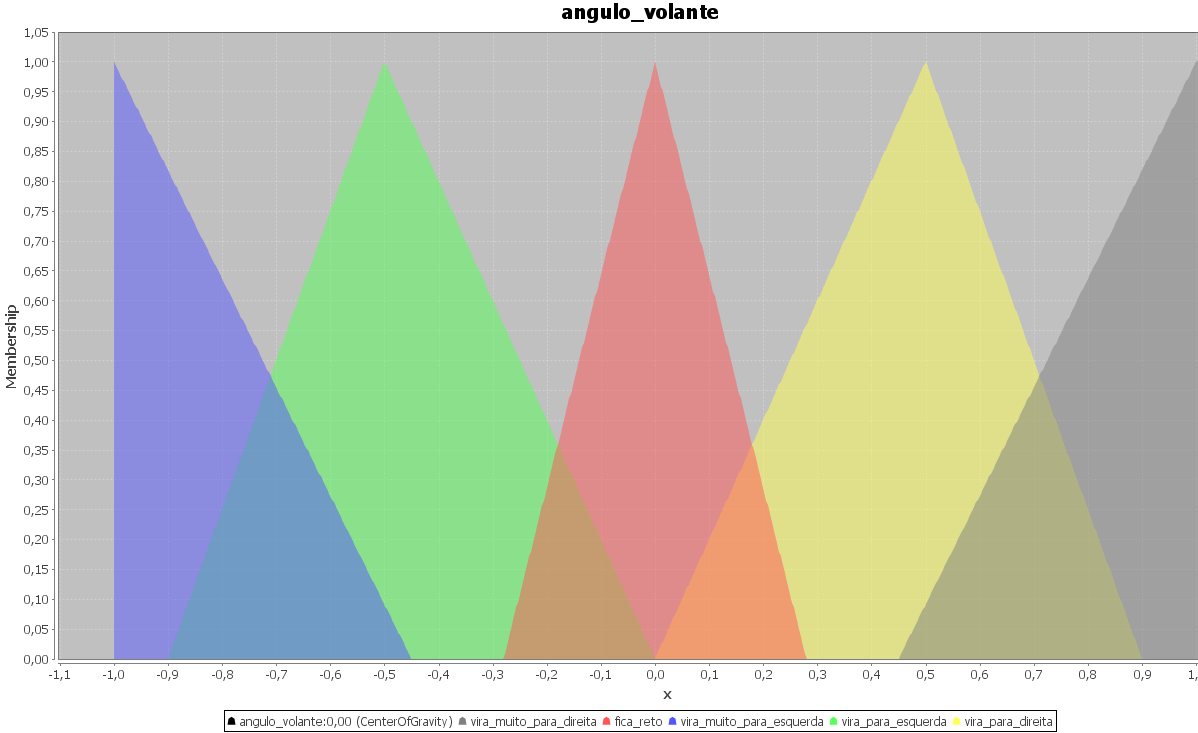
\includegraphics[width=\textwidth]{fig/angulo_volate.png}
    \caption{Gráfico de desfuzzyficação do ângulo de giro do volante do caminhão}
    \label{fig:axioms}
\end{figure}

\newpage
\section{Resultados}
O sistema, com os parâmetros definidos no código em anexo Fuzzy.fcl obteve resultados considerados razoáveis pela equipe, pois ele se mostrou estável e em raras situações teve resultados perfeitos ou resultados muito ruins. A seguir será apresentado algumas situações e o o respectivo comportamento do sistema.

\begin{figure}[H]
    \centering
    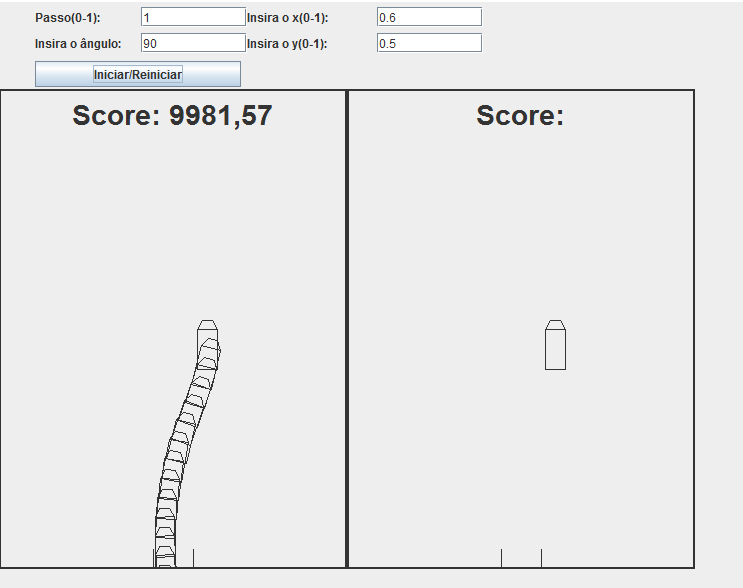
\includegraphics[width=\textwidth]{fig/resultado_2.png}
    \caption{Sistema se comportando perfeitamente em uma situação simples}
    \label{fig:axioms}
\end{figure}

\begin{figure}[H]
    \centering
    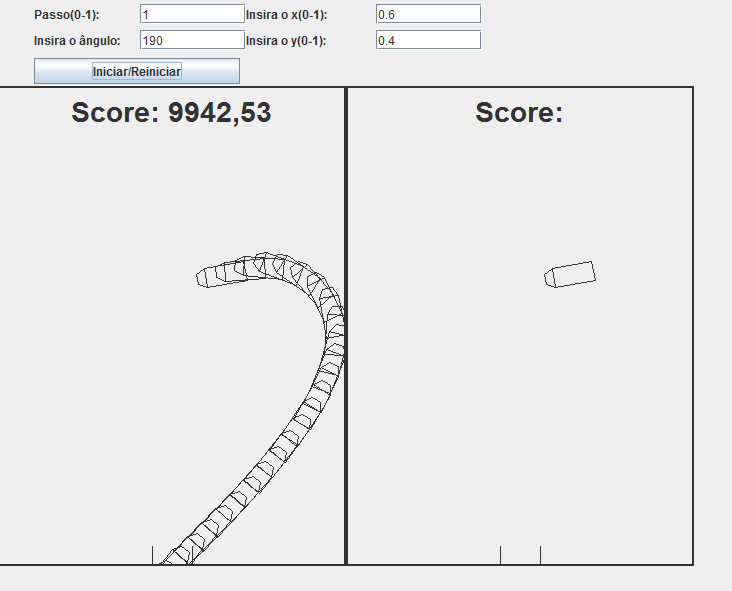
\includegraphics[width=\textwidth]{fig/resultado_1.png}
    \caption{Sistema conseguiu chegar a um resultado satisfatório mesmo saindo de uma posição adversa}
    \label{fig:axioms}
\end{figure}



\begin{figure}[H]
    \centering
    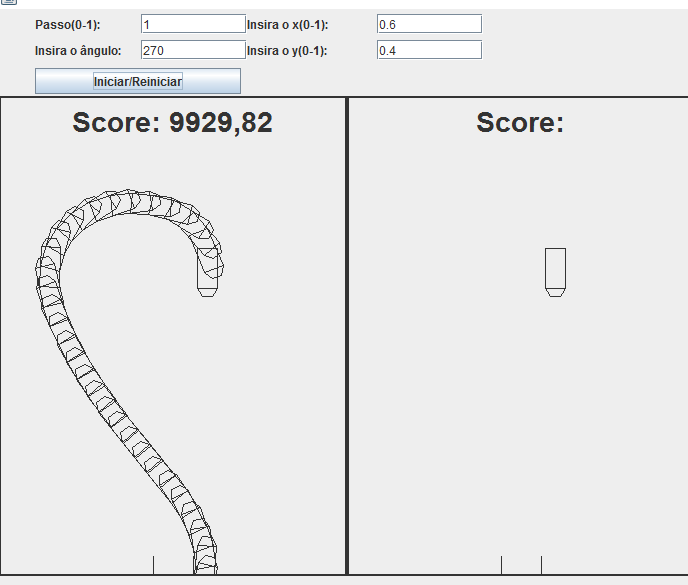
\includegraphics[width=\textwidth]{fig/resultado_3.png}
    \caption{Sistema conseguiu chegar a um resultado satisfatório mesmo saindo de uma posição extremamente adversa}
    \label{fig:axioms}
\end{figure}



\newpage
\section{Dificuldades}
A principal dificuldade da equipe foi encontrar os parâmetros e as formas que deveriam modelar as váriaveis a serem Fuzzyficadas. Essa dificuldade se dava pois uma modificação dos parâmetros gerava uma melhora signifcativa em algumas situações e, em outras, uma piora muito grande. Apesar de tentativas terem sido feitas, adicionando estados nas variáveis a serem fuzzyficadas, o sistema se tornou muito complexo e não houve melhora perceptível. Dessa forma, foi mantido uma forma mais simples e que gera um desempenho satisfatório.


\newpage
\section{Código}
O código da equipe está abertamente disponível no
\href{https://github.com/andrei258258/ine5430-fuzzy}{repositório da equipe}.


%%%%%%%%%%%%%%%%%%%%%%%%%%%%%%%%%%%%%%%%%%%%%%%%%%%%%%%%%%%%%%%%%%%%%%%%
%  ____  _ _     _ _       
% | __ )(_) |__ | (_) ___  
% |  _ \| | '_ \| | |/ _ \ 
% | |_) | | |_) | | | (_) |
% |____/|_|_.__/|_|_|\___/ 

\newpage
\begin{thebibliography}{9}

\bibitem{jfuzzy} 
http://jfuzzylogic.sourceforge.net/html/index.html - Acessado em 09 de novembro de 2017.

\bibitem{fcl}
http://ffll.sourceforge.net/fcl.htm - Acessado em 09 de novembro de 2017.

\bibitem{fuzzytruck}
http://rorchard.github.io/FuzzyJ/FuzzyTruck.html - Acessado em 09 de novembro de 2017.

\end{thebibliography}
%%%%%%%%%%%%%%%%%%%%%%%%%%%%%%%%%%%%%%%%%%%%%%%%%%%%%%%%%%%%%%%%%%%%%%%%

\end{document}